\chapter{結論與未來展望}

本章節將點出五個實驗中所有值得的想法,各個實驗中的缺陷也會在本章節總結,另外,仍有研究潛力的方向,像是 attention gate 參數調整、樂器資料集的拓展、loss 函數調整等等,這些會歸納在本章的未來展望中。

\section{結論}

由上章所有實驗的效果可以歸結出下列結論:
\begin{itemize}
    \item[1.] 實驗一的結果可以知道,直接使用 U-Net 輸出的頻譜與混音軌的相位直接合併輸出,會導致相位無法對應,進而導致輸出的音訊效果不好。但若使用輸出的所有頻譜作出 ratio mask filter 或是 Wiener filter,直接對混音軌的 STFT 做濾波,可以避免相位無法對應的問題,也可以確保輸出的音量可以與原本一致。
    \item[2.] 實驗二的結果可以知道,對 U-Net 輸出的頻譜做頻譜刪減法,可有小幅度的增進效能,降低主唱軌與伴奏軌相互干擾的問題。
    \item[3.] 實驗三的實驗可以知道,U-Net 模型在長片段的聲音中,不易找到相同聲音樣式的聲音(有規則、有頻率出現的聲音訊號,如:鼓聲、節奏吉他...等),但加上注意力機制後,可以明顯地將殘留在主唱預測音軌的鼓聲去除。
    \item[4.] 深度可分卷積與 inverted residual 可以有效地縮小 U-Net 模型,剪枝過後的模型仍保有聲音分離的能力,但 inverted residual 能力稍強,可以針對應用場域的需求做出調整。
    \item[5.] 模型皆可以有效的量化,代表此模型能在手機端使用,甚至可在實時的場域中作使用。
\end{itemize}


\section{未來展望}

U-Net 在聲音訊號分離仍有很多值得了解的面向。注意力模型 attention gate~\cite{oktay2018attention} 方法其中的 $\alpha$ 值目前為給定狀態,未來可測試不同參數,或是讓機器可以自主學習。針對模型剪枝方法(深度可分卷積~\cite{chollet2017xception,howard2017mobilenets}與 inverted residual~\cite{sandler2018mobilenetv2})導致的效果下滑,可對其再加上注意力機制 self-attention~\cite{shaw2018self} 或是 attention gate~\cite{oktay2018attention} 進行實驗。

上面談到是對模型改善的方法,另外可對其訓練資料—頻譜圖下手,比如 Spleeter~\cite{hennequin2020spleeter} 就想讓模型專注在人耳比較敏感的區域訓練即可,選擇以 1024 個 frequency bin 頻譜圖輸入至 U-Net 中訓練,這是在人耳敏感度、模型專注度與模型預測時間各方的調整,輸入頻譜圖越小可以讓模型預測時間更快,實時應用的緩衝更小。liu~\cite{liu2020channel} 提到的「channel-wise sub-band input」也是基於不同的頻段使用不同的模型架構對症下藥,不只可以縮小模型所需的參數,也可讓模型專注在各自的頻段上讓效果更好,也值得未來探討。

本論文基於的 U-Net 架構上有一個短版,也就是無法利用聲音訊號中的相位資訊,這也是 Demucs~\cite{defossez2019music} 所想要克服的問題,其用到了 LSTM~\cite{gers1999learning} 對時間序列的資訊取得做優化,但可能導致運算量增加或是運算時間無法因卷積的優勢降低。對此,Giri~\cite{giri2019attention} 提出的「Attention wave-u-net」可以解決此問題,將 LSTM 以 attention 替換值得在未來的實驗中探討。或是在 STFT 域中,使用二維卷積的 U-Net 訓練,對此,Choi 等人~\cite{choi2018phase} 提出的「Phase-aware speech enhancement with deep complex u-net」值得研究,直接使用 STFT 之後的值,而非單取其 Magnitude 成為模型的輸入,讓模型學習相位的變化。

% 在 loss 函數上也可有很多著墨點
不只針對 U-Net 上的優化,loss 函數也是一個值得研究的方向。一個好的 loss 函數幫助整個深度神經網路,在本論文中的所有模型採用 smooth L1 loss 函數,但是否能使用這邊採取的評估指標 SDR、SIR 與 SAR 作為 loss 函數?Nakajima~\cite{nakajima2018monaural} 等人提出了可能性,其將深度神經網路的輸出以 SDR 計算其與正確的訊號之間的 loss,在最後的評估時也取得了更好的成績。另外,Braun~\cite{braun2020consolidated} 等人與 gusó 的碩士論文~\cite{guso2020on_loss_functions} 針對語音強化(speech enhancement)與音樂分離領域做了一個完整的討論,將所有可以在監督式學習的 loss 函數列出,在未來可參考此研究,找到本架構最適合的 loss 函數。

% 頻譜刪減法在 nn 上實現
% 其他模型在 svs 上的應用可能
頻譜刪減法的討論,可參考在 Rohman~\cite{rohman2016novel} 等人的研究。非 U-Net 架構在音樂分離領域上的可能性,Tzinis~\cite{tzinis2020improving} 等人提出利用聲音辨別系統幫助聲音分離架構,Samuel~\cite{samuel2020meta} 等人提出利用 Meta-learning 方法幫助聲音分離架構。

% slakh2100 資料集以擴充各個樂器的資料
在資料的處理上面,為了之後其他樂器音軌的分離,需要拓展現有的資料,slakh2100~\cite{manilow2019cutting} 裡有需多高品質混音的樂器聲音,還有如何對資料做 augmentation 可以參考 Uhlich~\cite{uhlich2017improving} 等人的研究。

在模型預測能力與時間需求上,與其他模型來做比較如下圖。其中圖\ref{pic_conclusions1} 是代表訓練過程中,對於一秒的聲音,大約需要多少時間。圖\ref{pic_conclusions2} 是代表一秒的聲音分離時,加上檔案讀寫的時間,平均需要多少時間。由此可見,雖然 Spleeter 使用的 frquency-based 模型的分離速度的確很快,比起 Demucs 使用的 time-based 模型快很多,雖然本研究也是使用 frequency-based 模型,分離效果不錯但在速度上太過緩慢。未來研究中,調控 encoder 與 decoder 的層數,在效能與速度上取得平衡。

\begin{figure}[htbp]
    \hfil
    \begin{minipage}[t]{0.45\textwidth}
        \centering
        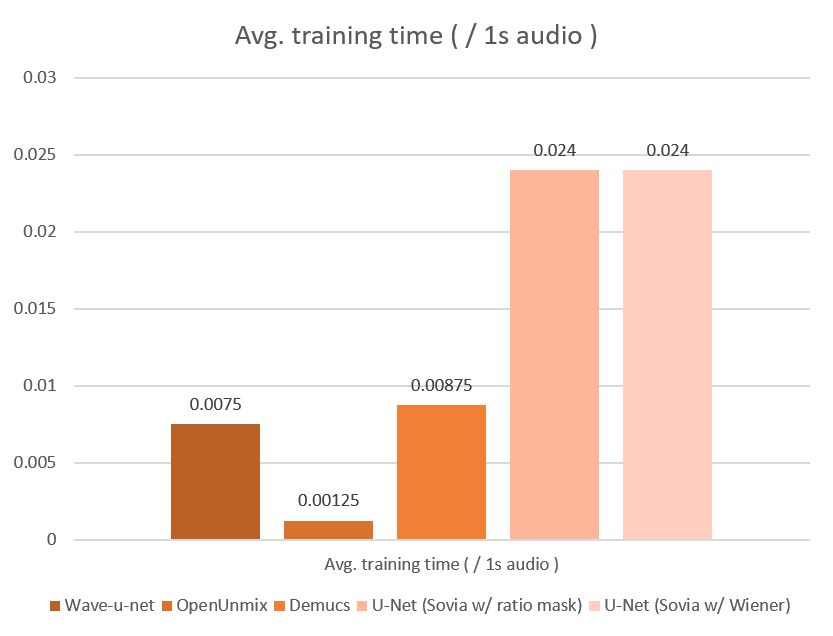
\includegraphics[width=\textwidth]{./figures/chapter06_conclusions/pic_conclusions1.png}
        \caption {一秒聲音需訓練的時間}
        \label{pic_conclusions1}
    \end{minipage}
    \begin{minipage}[t]{0.45\textwidth}
        \centering
        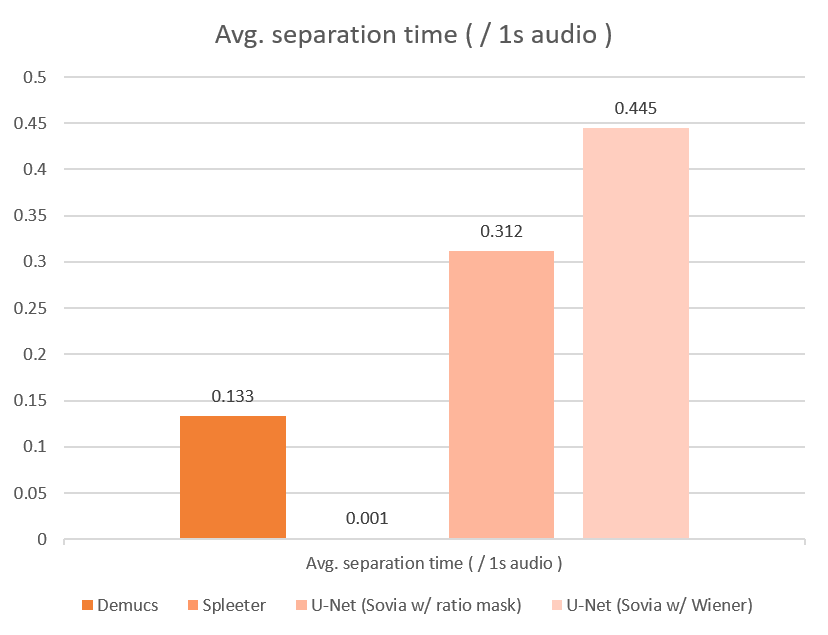
\includegraphics[width=\textwidth]{./figures/chapter06_conclusions/pic_conclusions2.png}
        \caption {一秒聲音平均分離的時間}
        \label{pic_conclusions2}
    \end{minipage}
    \hfil
\end{figure}